\section{Como agregar un nuevo experimento y hacerlo visible desde la interfaz gr�fica}

Un experimento es una clase que contiene una lista de algoritmos para resolver un problema espec�fico. Los algoritmos que conforman el experimento deben ser de un mismo tipo, por ejemplo, que la lista tenga instancias ``n'' repeticiones del Algoritmo Gen�tico. Actuando ``n'' como el n�mero de ejecuciones independientes del algoritmo. En la Figura \ref{fig:metaheuristics_extendido}, se muestra las interfaces del m�dulo de metaheur�sticas extendido.

\begin{figure}[H]
    \centering
    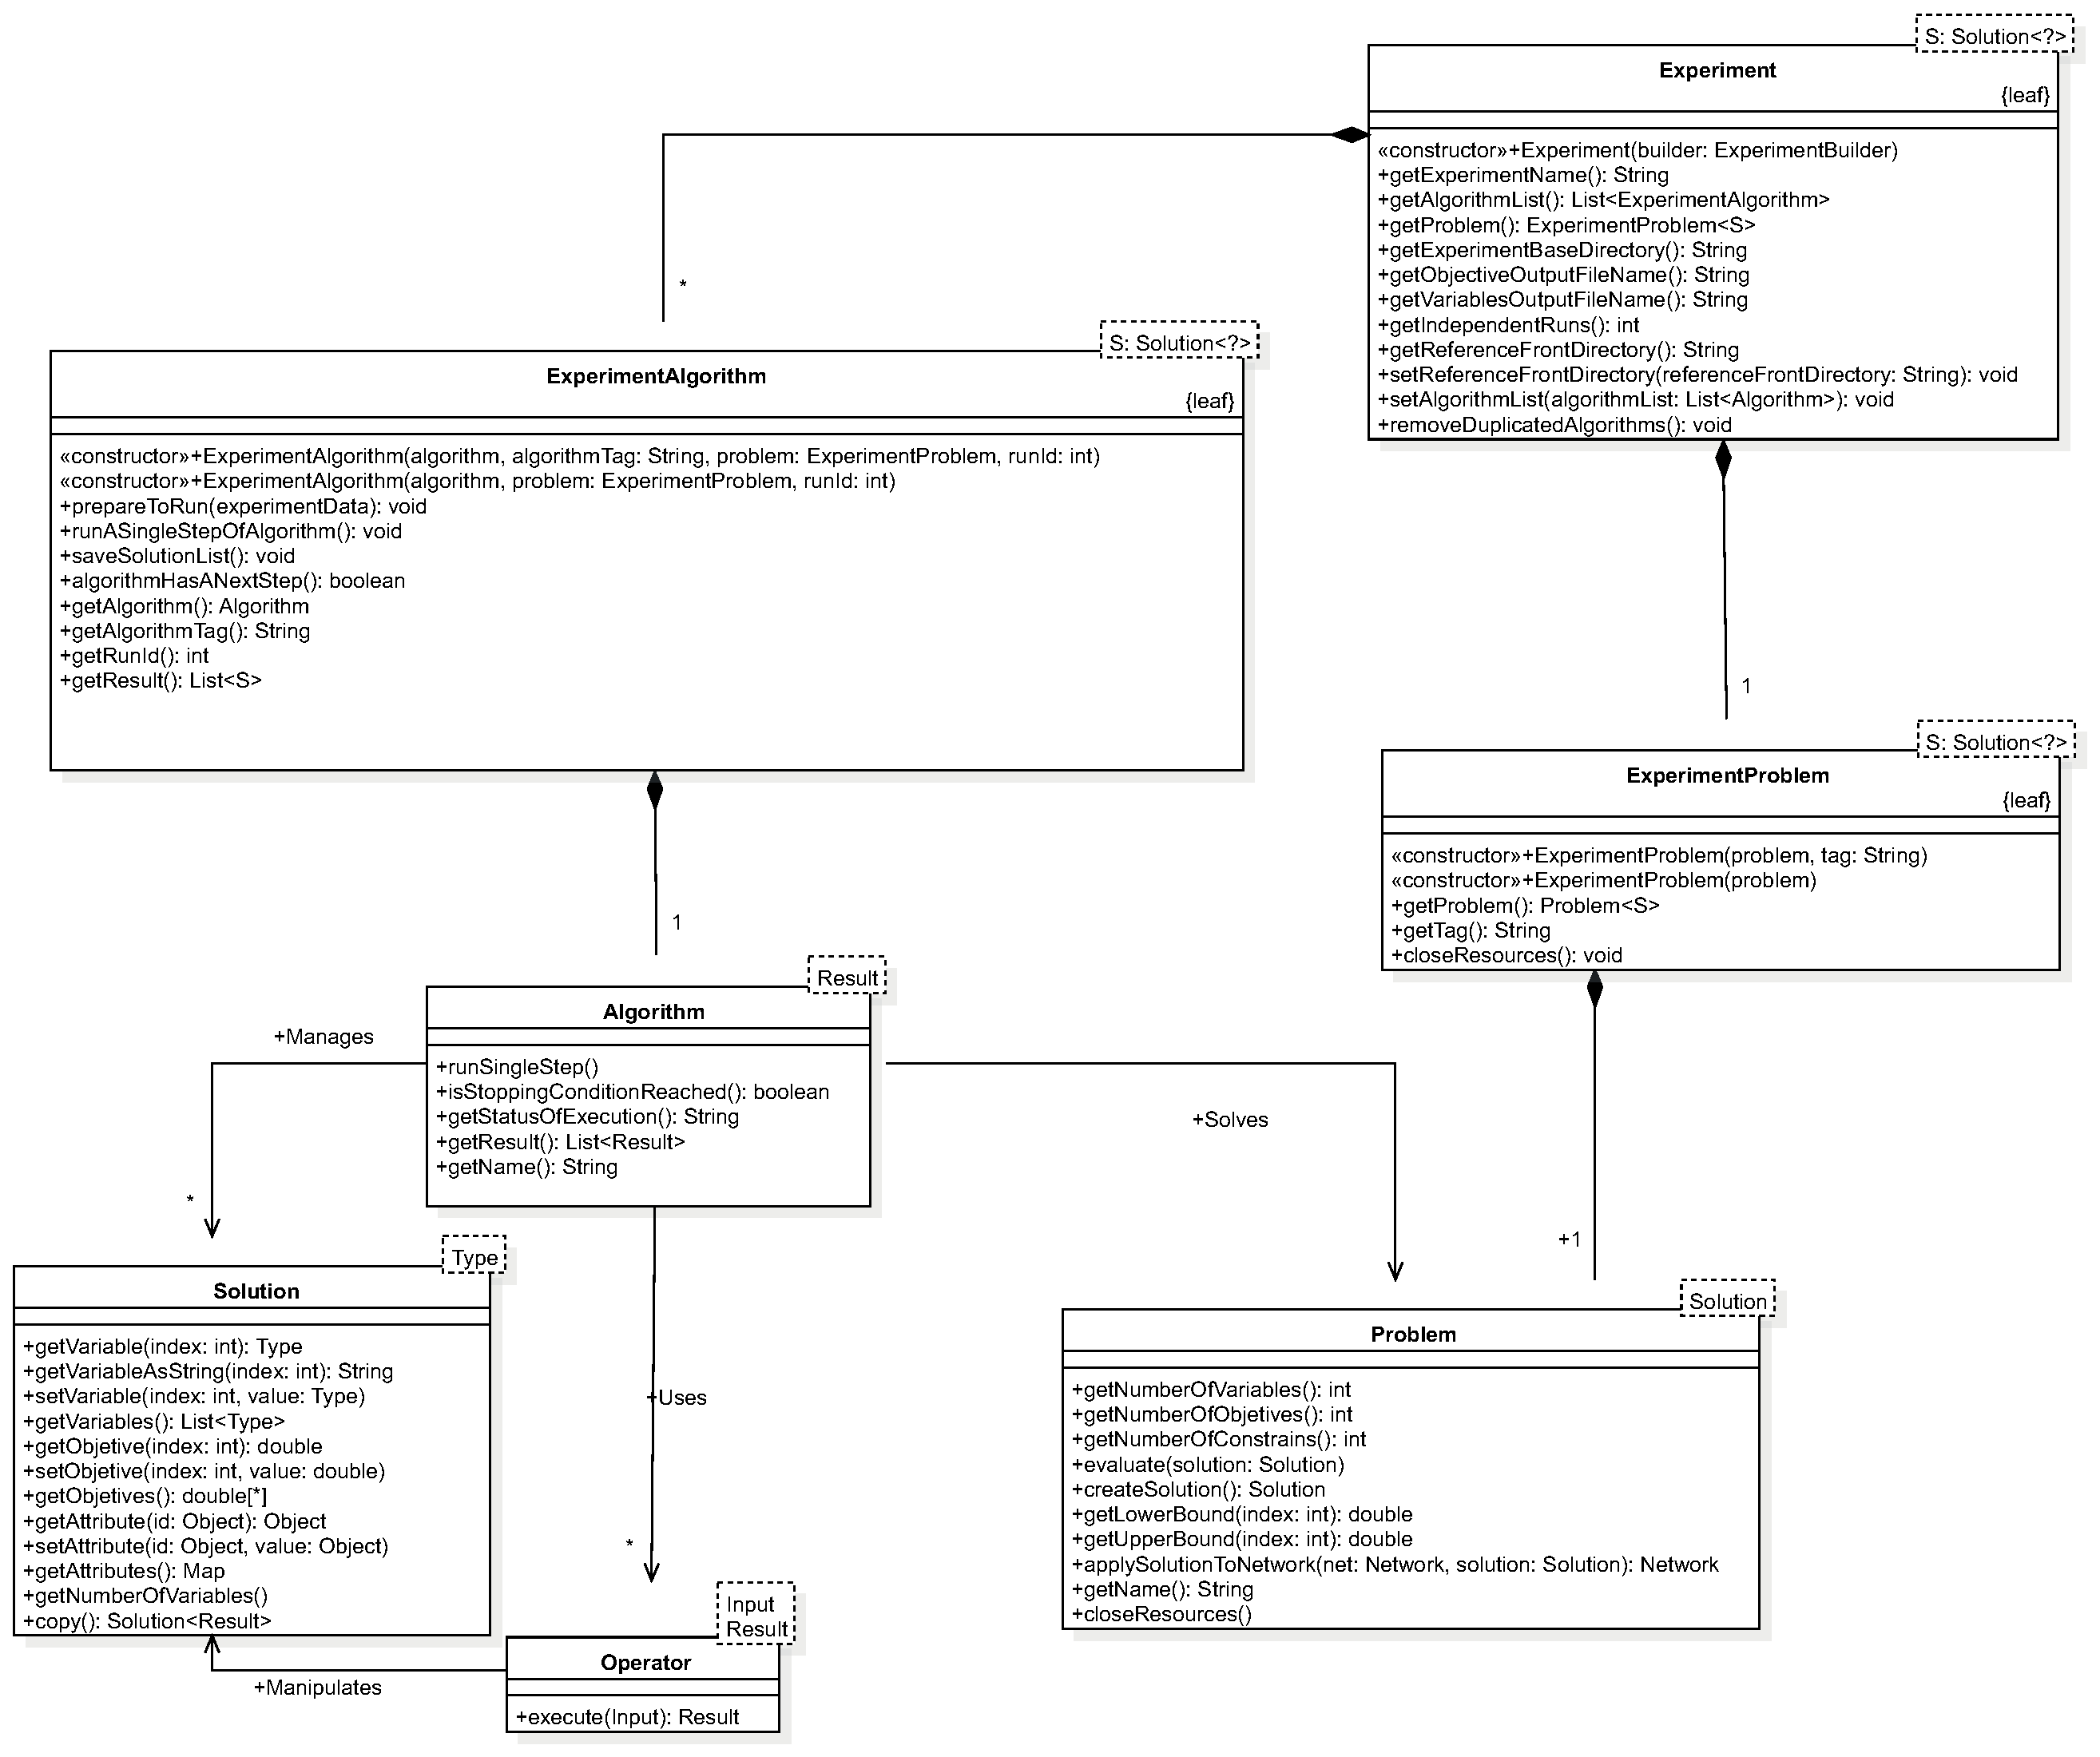
\includegraphics[width=\textwidth]{Seccion4/assets/d_class_metaheuristics_extendido.eps}
    \caption{Diagrama m�dulo metaheur�stica extendido.}
    \label{fig:metaheuristics_extendido}
\end{figure}

Para crear el experimento la aplicaci�n cuenta con una clase llamada \textit{ExperimentBuilder}.
Los par�metros \textit{ExperimentBaseDirectory} y \textit{ReferenceFrontDirectory} solo tienen uso en experimentos multiobjetivos. \textit{ExperimentBaseDirectory} indica donde guardar la frontera de Pareto de cada repetici�n del algoritmo multiobjetivo. En cambio, \textit{ReferenceFrontDirectory} indica donde guardar la frontera de Pareto final, que se obtiene al unir las fronteras de cada repetici�n y extraer solamente las soluciones no dominadas de dicho conjunto. 

\section{Interfaz Registrable}

Esta interfaz declara el m�todo \textit{build} y \textit{getParameters}. La declaraci�n del m�todo \textit{build}  corresponde a la siguiente:

\begin{lstlisting}
    R build(String inpPath) throws Exception;
\end{lstlisting}

Donde R corresponde al tipo de valor devuelto por la funci�n.

De esta clase se heredan dos subinterfaces. La primera corresponde a \textit{SingleObjectiveRegistrable} que debe ser usada para implementar los problemas monoobjetivos. En cuanto a la segunda, esta corresponde a \textit{MultiObjectiveRegistrable}, la cual se debe usar para los problemas multiobjetivos. El m�todo build sobreescrito por estas clases tiene la siguiente asignatura: 

\begin{lstlisting}
    Experiment<?> build(String inpPath) throws Exception;
\end{lstlisting}

\noindent %% remueve la identaci�n
donde \textit{Experiment} consiste en una clase que almacena una lista de algoritmos (Del mismo tipo) y el problema a resolver por estos algoritmos.

Las nuevas clases deben implementar la interfaz \textit{SingleObjectiveRegistrable} o \textit{MultiObjectiveRegistrable}, dependiendo del tipo de problema a tratar. Las clases que implementen cualquiera de estas dos interfaces deben ser guardados en una estructura de datos, la cual ser� recorrida cuando se inicie la ejecuci�n del programa y analizada usando la \textit{Java Reflection API}. Este an�lisis consistir� en escanear y validar el cumplimiento de la convenci�n establecida para las clases que implementan est� interfaz. Esta convenci�n consiste en lo siguiente:

\begin{itemize}
    \item La clase debe contener un �nico constructor que use la anotaci�n \textit{@NewProblem.}
    \item Si el constructor requiere par�metros �stos deben estar descritos usando la anotaci�n \textit{@Parameters.}
    \item El constructor debe declarar los par�metros en el siguiente orden, de acuerdo con su tipo.
    \begin{enumerate}
        \item Object: Usado para inyectar los operadores. �stos pueden posteriormente ser casteados a su tipo correcto. La anotaci�n correspondiente es \textit{@OperatorInput}
        \item File: Usados cuando el problema requiere informaci�n adicional que se encuentra en un archivo diferente. La anotaci�n correspondiente es \textit{@FileInput}
        \item int, Integer, double o Double: Usado generalmente para configurar valores en el algoritmo o si el problema requiere otros valores que no fueron solicitados al crear los operadores. Las anotaciones correspondientes son \textit{@NumberInput y @NumberToggleInput.}
        \item El constructor debe solicitar la misma cantidad de par�metros que las descritas en la anotaci�n \textit{@Parameters.}
    \end{enumerate}
\end{itemize}

Si estas convenciones no se cumplen, entonces un error en tiempo de compilaci�n ser� emitido como se mencion� anteriormente en la secci�n anterior.

El orden en el que son inyectados los par�metros consiste en el siguiente:

\begin{enumerate}
    \item Par�metros descritos por \textit{@OperatorInput}
    \item Par�metros descritos por \textit{@FileInput}
    \item Par�metros descritos por \textit{@NumberInput}
    \item Par�metros descritos por \textit{@NumberToggleInput}
\end{enumerate}

Una vez que se haya configurado el problema a trav�s de la interfaz se crear� la instancia de la clase que hereda de Registrable y se llamar� a su m�todo build, para crear el experimento y comenzar su ejecuci�n.

La estructura de datos para registrar las clases que heredan de \textit{SingleObjectiveRegistrable} y \textit{MultiObjectiveRegistrable} se encontrar� en la clase \textit{RegistrableConfiguration}.


A continuaci�n de define detalladamente cada una de las anotaciones permitidas en la clase Registrable.


\subsection{\textit{@NewProblem}}
Esta anotaci�n permite indicar el nombre del problema que ser� mostrado en la interfaz gr�fica. Puedes ver el uso de esta anotaci�n en la Figura \ref{fig:constructor_heredado_registrable}.

\begin{figure}[H]
    \centering
    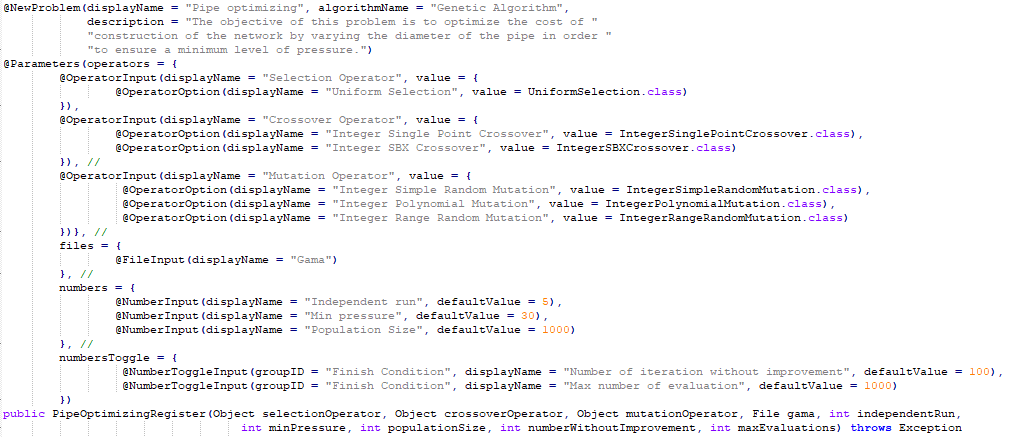
\includegraphics[width=0.98\textheight, angle=90]{Seccion4/assets/ConstructorHeredadoRegistrable.png}
    \caption{Constructor de clase que hereda de registrable y sus metadatos para cada par�metro.}
    \label{fig:constructor_heredado_registrable}
\end{figure}

Los elementos en esta anotaci�n consisten en:
\begin{itemize}
    \item \textit{displayName}: El nombre del problema. Este nombre tambi�n act�a como el nombre de la categor�a.
    \item \textit{algorithm}: Un \textit{String} con el nombre del algoritmo usado para resolver el problema.
    \item \textit{description}: Un \textit{String} con la descripci�n del algoritmo.
\end{itemize}

El nombre dado en el elemento \textit{displayName}, es el nombre visible del problema en el men� de la aplicaci�n y permite agrupar a los problemas que tengan el mismo nombre, pero distintos algoritmos, como se ve en la Figura \ref{fig:menu_del_problema}.

\begin{figure}[H]
    \centering
    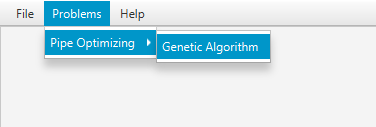
\includegraphics[width=\textwidth]{Seccion4/assets/MenuDelProblema.png}
    \caption{Men� de problemas.}
    \label{fig:menu_del_problema}
\end{figure}

Esta anotaci�n solo puede estar en un constructor, en caso de que esta anotaci�n no est� presente, un error en tiempo de ejecuci�n ser� lanzado. 

\subsection{\textit{@Parameters}}
Esta anotaci�n permite agregar informaci�n acerca de los par�metros recibidos por el constructor. Cuando el constructor tiene esta anotaci�n, por convenci�n, est� obligado a declarar los par�metros en un orden determinado en base a tu tipo. Este orden es el siguiente:

\begin{enumerate}
    \item \textit{Object}
    \item \textit{File}
    \item \textit{int} o \textit{double}
\end{enumerate}

Si el constructor no declara los par�metros en ese orden un error en tiempo de ejecuci�n ser� lanzado.

Dentro de esta anotaci�n existen varios elementos. Estos elementos son:
\begin{itemize}
    \item \textit{operators}: Arreglo que recibe anotaciones del tipo \textit{OperatorInput}. 
    \item \textit{files}: Arreglo que recibe anotaciones del tipo \textit{FileInput}.
    \item \textit{numbers}:  Arreglo que recibe anotaciones del tipo \textit{NumberInput}.
    \item \textit{numbersToggle}: Arreglo que recibe anotaciones del tipo \textit{NumberToggleInput}.
\end{itemize}

El valor por defecto para todos los elementos mencionados anteriormente es un arreglo vac�o (\{\}).
No usar la anotaci�n \textit{@Parameters} tiene el mismo efecto que usar la anotaci�n, pero con sus valores por defecto.

Puede ver el uso de esta anotaci�n en la Figura \ref{fig:constructor_heredado_registrable}. 

\subsection{\textit{@OperatorInput}}
Esta anotaci�n agrega informaci�n a uno de los par�metros del constructor acerca de los posibles operadores que pueden ser recibidos por ese par�metro. 
Dentro de esta anotaci�n existen varios elementos. Estos elementos son:
\begin{enumerate}
    \item \textit{displayName}: Nombre de categor�a para los operadores.
    \item \textit{value}: Arreglo que recibe anotaciones del tipo \textit{OperatorOption}.
\end{enumerate}

En la ventana de configuraci�n de problema, estos par�metros son vistos con un \textit{ComboBox} como muestra la Figura \ref{fig:componente_operator_input}. 

\begin{figure}[H]
    \centering
    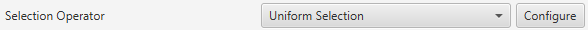
\includegraphics[width=\textwidth]{Seccion4/assets/ComponenteOperatorInput.png}
    \caption{Componente \textit{ComboBox} para configurar los operadores.}
    \label{fig:componente_operator_input}
\end{figure}

Las alternativas disponibles dentro del \textit{ComboBox} est�n dadas por aquellas indicadas en el elemento value de este operador. Como se muestra en la Figura \ref{fig:constructor_heredado_registrable}, la �nica alternativa para el \textit{Selection Operator} es el operador \textit{UniformSelection} apreciado en la Figura \ref{fig:componente_operator_input_expandido}.
 
\begin{figure}[H]
    \centering
    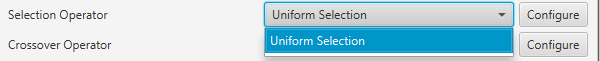
\includegraphics[width=\textwidth]{Seccion4/assets/ComponenteOperatorInputExpandido.png}
    \caption{\textit{ComboBox} expandido para configurar el operador.}
    \label{fig:componente_operator_input_expandido}
\end{figure}

Por defecto, el \textit{ComboBox} selecciona el primer elemento de la lista.
El bot�n \textit{Configure} permite configurar los par�metros que recibe el constructor del operador, aquel que posee la anotaci�n \textit{@DefaultConstructor}. Para el caso del operador \textit{UniformSelection}, su interfaz de configuraci�n se muestra en la Figura~\ref{fig:interfaz_uniform_selection}.

\subsection{\textit{@OperatorOption}}
Esta anotaci�n permite indicar las alternativas de operadores que puede recibir un par�metro para una categor�a de operador indicada por la anotaci�n \textit{@OperatorInput}.
Dentro de esta anotaci�n existen varios elementos. Estos elementos son:
\begin{itemize}
    \item \textit{displayName}: Nombre del operador. Este es el nombre visualizado en el \textit{ComboBox} como se muestra en la Figura \ref{fig:componente_operator_input_expandido}.
    \item \textit{value}: Instancia del tipo \textit{Class} que referencia el tipo de operador.
\end{itemize}


\subsection{\textit{@FileInput}}
Esta anotaci�n indica que hay un par�metro que espera recibir un objeto de tipo \textit{File}. Cuando esta anotaci�n est� presente junto con su par�metro, en la interfaz, aparecer� un apartado que abre un \textit{FileChooser} o un \textit{DirectoryChooser} para buscar un archivo o directorio, respectivamente.
Dentro de esta anotaci�n existen varios elementos. �stos son:
\begin{itemize}
    \item \textit{displayName}: Nombre del par�metro. Este nombre tambi�n corresponde al nombre visualizado en la ventana de configuraci�n como se muestra en la Figura \ref{fig:componente_file_input}.
    \item \textit{type}: Indica el modo en que se abrir� el \textit{\textit{FileChooser}}. Este elemento recibe un enumerado del tipo \textit{Type}; los cuales son \textit{Type.OPEN}, \textit{Type.SAVE}, que abren un \textit{FileChooser} para leer o guardar un archivo; y \textit{Type.Directory}, el cual abre un \textit{DirectoryChooser} para seleccionar un directorio. La opci�n por defecto es \textit{FileType.OPEN}.
\end{itemize}

\begin{figure}[H]
    \centering
    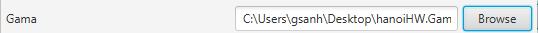
\includegraphics[width=\textwidth]{Seccion4/assets/ComponenteFileInput.png}
    \caption{Apartado para configurar el par�metro de tipo \textit{File}.}
    \label{fig:componente_file_input}
\end{figure}

Si el \textit{TextField} donde se muestra la ruta est� vac�o, es decir, no se ha seleccionado un archivo o carpeta, entonces ser� inyectado \textbf{\textit{null}} en el par�metro correspondiente del constructor.

\subsection{\textit{@NumberInput}}
Esta anotaci�n indica que hay un par�metro del tipo \textit{int} o \textit{double} o sus tipos envoltorios \textit{Integer} o \textit{Double}, respectivamente. Esta anotaci�n agrega en la interfaz un \textit{TextField} que solo permite como entrada un n�mero.  Si el tipo del par�metro es \textit{int} o \textit{Integer}, entonces el \textit{TextField} solo permite ingresar n�meros enteros. Por otro lado, si el par�metro es \textit{double} o \textit{Double}, entonces en la interfaz se acepta el ingreso de n�meros enteros o decimales. El apartado para esta anotaci�n se muestra en la Figura \ref{fig:componente_number_input}.

\begin{figure}[H]
    \centering
    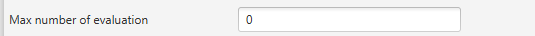
\includegraphics[width=\textwidth]{Seccion4/assets/ComponenteNumberInput.png}
    \caption{\textit{TextField} presente cuando est� la anotaci�n \textit{@NumberInput}.}
    \label{fig:componente_number_input}
\end{figure}

Dentro de esta anotaci�n existen los siguientes elementos:
\begin{itemize}
    \item \textit{displayName}: Nombre del par�metro.
    \item \textit{defaultValue}: Valor por defecto de la propiedad. Si el tipo de par�metro en el constructor de la clase que hereda de \textit{Registrable} es un entero, pero se ingresa como valor por defecto un n�mero con decimales, los decimales ser�n truncados. Si este elemento no se define su valor por defecto es 0.
\end{itemize}

\subsection{\textit{@NumberToggleInput}}
Esta anotaci�n indica que hay un conjunto de par�metros que son mutuamente excluyentes entre ellos, es decir, que solo un par�metro puede recibir el valor. En la interfaz, el nombre del grupo aparece sobre los componentes. Dentro de un mismo grupo solo se puede configurar un par�metro. El par�metro por configurar debe ser indicado activando el \textit{ToggleButton} correspondiente, lo cual conlleva a la activaci�n del \textit{TextField}.
Dentro de esta anotaci�n existen varios elementos. Estos elementos son:
\begin{itemize}
    \item \textit{groudID}: \textit{String} con un id para el grupo. Las anotaciones \textit{NumberToggerInput} que tengan el mismo id, en la interfaz, se encuentran en una secci�n cuyo t�tulo es el nombre del grupo. Esto se aprecia en la Figura \ref{fig:componente_number_toggle_input}. 
    \item \textit{displayName}: Nombre del par�metro.
    \item \textit{defaultValue}: Valor por defecto de la propiedad. Si el tipo de par�metro en el constructor de la clase que hereda de \textit{Registrable} es un entero, pero se ingresa como valor por defecto un n�mero con decimales, los decimales ser�n truncados. Si este elemento no se define su valor por defecto es 0.
\end{itemize}

\begin{figure}[H]
    \centering
    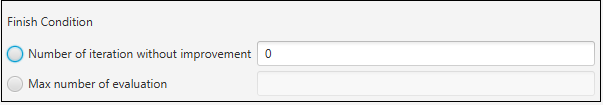
\includegraphics[width=\textwidth]{Seccion4/assets/ComponenteNumberToggleInput.png}
    \caption{Apartado para \textit{NumberToggleInput} con el mismo GroupID.}
    \label{fig:componente_number_toggle_input}
\end{figure}

El par�metro configurado en la interfaz de usuario recibe el valor indicado en el \textit{TextField}. Si el \textit{TextField} queda vac�o entonces recibe el valor cero. Sin embargo, los dem�s par�metros, cuyos \textit{TextField} est�n deshabilitados, van a recibir el valor \textbf{\textit{Double.MIN\_VALUE}}, si el par�metro es de tipo \textit{double} o \textit{Double}; o \textbf{\textit{Integer.MIN\_VALUE}} si el par�metro es de tipo \textit{int} o \textit{Integer}. Por ejemplo, en la Figura \ref{fig:componente_number_toggle_input}, se observa que el par�metro ``\textit{Number of iteration without improvement}'' esta activado, pero no contiene un valor, entonces al crear la instancia el constructor va a recibir el valor cero. Pero el par�metro ``\textit{Max number of evaluation}'', al no haber sido escogido, recibe el valor \textit{Integer.MIN\_VALUE}, puesto que este par�metro era de tipo \textit{int} o \textit{Integer}.

En la Figura \ref{fig:constructor_heredado_registrable} se puede ver el uso de la anotaci�n \textit{NumberToggleInput}. El componente que representa esta anotaci�n en la GUI se puede apreciar en la Figura \ref{fig:componente_number_toggle_input}. El groupID es usado para nombrar la secci�n. 

En el elemento \textit{numbersToggle} de la anotaci�n \textit{@Parameters}, las anotaciones que pertenezcan al mismo grupo deben estar continuas. En caso de que esto no se cumpla se lanza una excepci�n al momento de ejecutar la aplicaci�n.

Las anotaciones presentadas en las dos secciones anteriores deben ser usadas en constructores p�blicos.
